\documentclass[12pt]{article}
\usepackage[utf8]{inputenc}
\usepackage{float}
\usepackage{amsmath}


\usepackage[hmargin=3cm,vmargin=6.0cm]{geometry}
%\topmargin=0cm
\topmargin=-2cm
\addtolength{\textheight}{6.5cm}
\addtolength{\textwidth}{2.0cm}
%\setlength{\leftmargin}{-5cm}
\setlength{\oddsidemargin}{0.0cm}
\setlength{\evensidemargin}{0.0cm}

%misc libraries goes here
\usepackage{tikz}
\usetikzlibrary{automata,positioning}

\begin{document}

\section*{Student Information } 
Full Name : Furkan TAŞBAŞI \\ 	
Id Number : 2041853 \\		
\\	
Full Name : Batuhan BAT \\
Id Number : 2035707 \\

\section*{Graph}
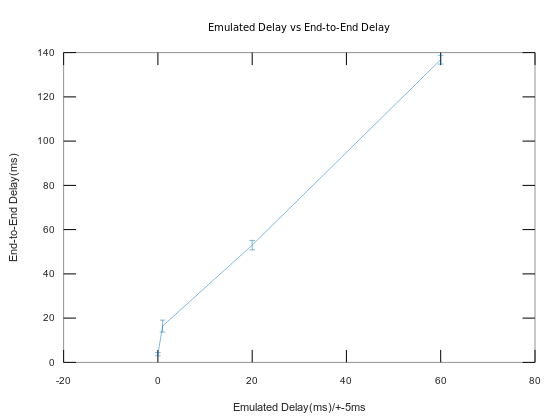
\includegraphics[height=360pt]{graph.png}

As we can recognize from the graph given above that there is a linear correspondence between network emulation delay and the end-to-end delay. Since emulated delay does not include queueing, transmission, propagation and routing delays, the slope of the graph is different from 1(one). Since queueing, transmission, propagation and routing delays are not major factors, even the slope of the graph is not 1(one), it is still linear.

\section*{Design}
First of all, before code process we designed our TCP and UDP server-client structures according to a data consisting of 100 bytes(characters). Source computer gets whole data from a file named "file.txt" 100 characters for each step. Then source creates a TCP connection to the broker and sends a data which compounds from 100 bytes to broker. Here source node has TCP client features. Then broker listens network via it's interface from source with TCP Server behavior. Whenever it takes a 100 bytes data, it starts to packetize it into 10 different packets by adding index information of single integer character to end of each packet which makes every packet sized of 11 character length(10 char's from message + 1 int from helper index). After packetizing process, broker sends all packets to routers with UDP client behavior. Routing from Broker to Router devices works according to a simple algorithm. If a packet has an odd sequence number as the helper index, it's forwarded to Router2 device otherwise(if the packet has an even number as the helper index) it is forwarded to Router1 device. Router devices directly behaves as if a bridge which listens network with a UDP server behavior and takes 11 characters length packets. Whenever a router takes a packet, it sends it to destination device with UDP client behavior. After all routing process, destination takes 110 bytes single data from network by listening its two different interfaces(Router1 and Router2) with UDP server behavior. After taking whole packets, it merges them all into a single big data by sorting 110 bytes of 10 different packets according to the helper index that exists at the end of all packets.In addition to that we recorded all delay starts(sending time data) to a file in source device and delay ends(arriving time data) to a file in destinaton device.

While measuring the end-to-end delays, we have seen such non-synchronized devices as a timestamp, we have used NTP(network time protocol) comments to  synchronize all devices. We have used "time.nist.gov" servers for this purpose. Then, we have validated that there is no clock difference between devices. 

\section*{Experiment}
While doing end-to-end delal experiments, we have sent 10(ten) different sets that each of them including 10(ten) packets and measured the average network delays as $3.7000000000$ ms, $16.4000000000$ ms, $53.0000000000$ ms, $136.8000000000$ ms for $0$ ms, $1$ ms, $20$ ms, $60$ ms in relative order. After that, we have calculated standart deviations of each experiment sets then applied them to the formula with corresponding confidence interval values step by step for all experiments. While applying the formula, we have multiplied average values with Z value (which is 1.96 for $.95$ confidence interval), then multiplied the sub result with the value of standart deviation divided by square root of sample size which is 10 ($\sqrt{n}$ where n is 10). As a result we have found confidence intervals as $0.718666666666663$, $2.7127104936248$, $2.14707242542028$, $1.9773454708551$ (in ms) respectively for experiments in relative order.
Finally, we draw a graph including these errors for all points.
\section*{Notification}
All homework processes(design,code implementation,configurations and graphs) are done together with both group members and GoogleDrive is used for version control for all homework.

\end{document}